\documentclass[11pt,letter]{article}
\usepackage[utf8x]{inputenc}
\usepackage{graphicx}
\usepackage{url}
\usepackage{amsmath}
\usepackage{amsfonts}

\title{Path-Selection in Floating Sensor Networks}
\author{Kevin Weekly}

\begin{document}

\maketitle

\begin{abstract}
This project will focus on a particular scenario of assigning floating sensors to paths through a river system.  The goal will be to maximize the combined spatial and temporal coverage of a river with a fixed number of units.  It is formulated as a 0-1 Integer Linear Program to be solved by standard solvers.

We begin by constructing the structure of the problem. First, the domain is seperated into regions, where each is given a unique label.  Also, a weight can be associated with each region corresponding to the value of sensing that region.  Then, a set of paths is enumerated by traversing the connectivity of the regions from a given source region and several sink regions.

From these paths, 0-1 Integer Linear Problem is built and optimal solutions found using the CPLEX and glpk solvers.  From the running time of the computation we can conclude that using this method is feasible for operational use and challenges the current practice of heuristic human decision.
\end{abstract}
\newpage
\tableofcontents

\section{Introduction}
This report is a part of UC Berkeley's Floating Sensor Network Project's\cite{fsnweb} continuing development of a fleet of 40 ``Generation 3'' motorized floating sensor units, or \emph{drifters}, to be used for collection of water quality in California's Sacramento--San Joaquin River delta (See Figure \ref{fig:domain}). 

\begin{figure}[ht]
\centering 
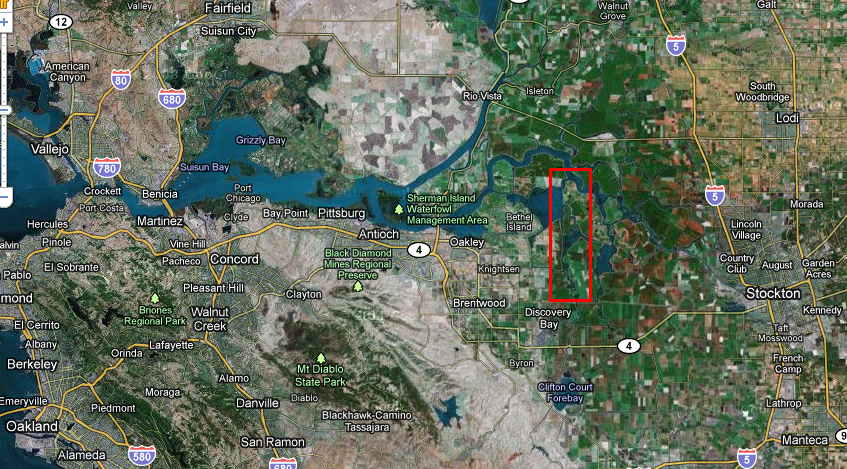
\includegraphics[width=1\linewidth]{figures/domain.png}
\caption{Operating region shown in red. Immediately west of map is San Francisco and the Pacific Ocean.\label{fig:domain}}
\end{figure}


The task of collecting most of the data in this environment currently falls under the responsibility of a sparse set of fixed-location sensor stations distributed throughout the domain.  Through complex models, the water speed, depth, and salinity readings from these stations give a good indication of mass flow through the system. However, the same information at the detail level of tributaries and lakes remains hazy. Many more locations must be sensed to obtain observability at this level. Hence there is a need for sensors with dynamic location.

\begin{figure}[ht]
\centering 
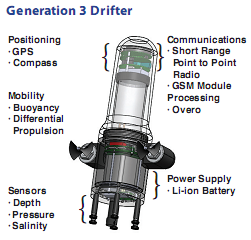
\includegraphics[width=0.5\linewidth,trim=0 0 0 20px,clip=true]{figures/drifter.png}
\caption{A ``Generation 3'' motorized floating sensor unit.\label{fig:gen3}}
\end{figure}

Figure \ref{fig:gen3} illustrates the high-level systems of our drifter units. Of note are the propulsion capabilities of the unit allowing some authority over its dynamics.  Also onboard is a highly-capable embedded Linux computer and means of communication to a central coordinator.  With intelligent coordination of their movements, we will be able to use a fleet of such units to instrument a large area much more economically than a fixed-location deployment.

\section{Problem Statement}


\section{Region Labelling}
\cite{floodfill}

\section{Path enumeration}

\section{}

\section{Conclusion}


\bibliographystyle{ieeetr}
\bibliography{cites}


\end{document}
